\documentclass[12pt]{article}
\usepackage[english]{babel}
\usepackage{natbib}
\usepackage{url}
\usepackage[utf8x]{inputenc}
\usepackage{amsmath}
\usepackage{graphicx}
\graphicspath{{images/}}
\usepackage{parskip}
\usepackage[includeheadfoot,margin=1.0in]{geometry}
\usepackage{fancyhdr}
%\usepackage[letterpaper, portrait, margin=1.0 in]{geometry}
\usepackage{fixme}

\title{GRIP Computer Vision Program}
\author{Thomas Clark}
\date{\today}

\makeatletter
\let\thetitle\@title
\let\theauthor\@author
\let\thedate\@date
\makeatother

\fxsetup{
    status=draft,
    author=,
    layout=inline,
    theme=color
}

\pagestyle{fancy}
\fancyhf{}
\lhead{\thetitle}
\cfoot{\thepage}

\begin{document}

%%%%%%%%%%%%%%%%%%%%%%%%%%%%%%%%%%%%%%%%%%%%%%%%%%%%%%%%%%%%%%%%%%%%%%%%%%%%%%%%%%%%%%%%%

\begin{titlepage}
    \centering
    
\includegraphics[scale = 0.25]{wpi.png}\\[1.0 cm]
    \textsc{\LARGE Worcester Polytechnic Institute}\\[1.0 cm]
    \textsc{\Large Major Qualifying Project}\\[0.5 cm]
    \rule{\linewidth}{0.2 mm} \\[0.4 cm]
    { \huge \bfseries \thetitle}\\[0.4 cm]
    { \large Graphically Represented Image Processing}\\
    \rule{\linewidth}{0.2 mm} \\[1.0 cm]

    \begin{flushleft}
        \emph{Submitted By:}\\
        Thomas Clark, Computer Science\\
        [0.4 cm]
        \emph{Advised By:}\\
        Michael Gennert, Robotics Engineering Director and Computer Science Professor\\
        Brad Miller, Robotics Engineering Professor\\[2 cm]
       \end{flushleft}

    {\large \thedate}\\[2 cm]

    \vfill

\end{titlepage}

%%%%%%%%%%%%%%%%%%%%%%%%%%%%%%%%%%%%%%%%%%%%%%%%%%%%%%%%%%%%%%%%%%%%%%%%%%%%%%%%%%%%%%%%%

\tableofcontents
\pagebreak

%%%%%%%%%%%%%%%%%%%%%%%%%%%%%%%%%%%%%%%%%%%%%%%%%%%%%%%%%%%%%%%%%%%%%%%%%%%%%%%%%%%%%%%%%

\section{Introduction}
Computer vision is an important field in robotics and computer science.  It is used by many groups, from research labs to competitive high school robotics teams.  Unfortunately, tasks involving computer vision are difficult to approach without prior experience with the field as well as the languages and toolkits commonly used.
\par
Teams participating the FIRST Robotics Competition are often presented with challenges requiring the use of computer vision to gain extra points in a match.  To aid in this, students are provided access to industry-grade computer vision toolkits, such as the Open Source Computer Vision Library and the NI Vision software.  However, the six-week build season required by FRC makes it infeasible for many teams to invest time in learning new programming languages, studying APIs, and experimenting with algorithms and parameters.  For this reason, the vision challenges are typically attempted by only the small portion of veteran teams who have the advantage of having adult mentors with computer vision experience.  As a result, many students who are interested in robotics and programming are not exposed to computer vision.
\par
Previous projects have been successful in providing tools for FIRST Robotics Competition participants to pass the barrier to entry for difficult computer programming tasks.  For example, the WPI project RobotBuilder provides a graphical user interface for generating robot control system code templates.  The RobotBuilder program allows students with little or no previous knowledge of the WPI Robotics Library to use a simple, intuitive UI to specify details about a robot's hardware, and generates code that can serve as a starting point for a team's robot software.  This has significantly improved the user experience of writing robotics software with the WPI Robotics Library, and since its release in 2013 the portion of teams using the library has increased significantly.  A related program that allows students to graphically compose computer vision algorithms could similarly increase the exposure to computer vision.
\par
Although FIRST was the initial motivation for this project, computer vision researchers could also benefit from a graphical tool like this.  The process of adjusting an algorithm, recompiling, and re-running a program results in a slow feedback loop where there is a significant delay between a programmer making changes and the programmer seing the results.  There's room for improvement in this process.  Development of new algorithms would be sped up if the developers could see the results in real-time as they change the parameters.

%%%%%%%%%%%%%%%%%%%%%%%%%%%%%%%%%%%%%%%%%%%%%%%%%%%%%%%%%%%%%%%%%%%%%%%%%%%%%%%%%%%%%%%%%

\section{Background and Motivation}
Computer vision is traditionally implemented by sending an image though a processing pipeline, where each step transforms the output of the previous step into a more abstract piece of data, such as a list of edges or the location of a feature.  It has many applications in robotics and other fields.  However, vision is a complex enough concept that each computer vision problem essentially requires a completely different set of steps and parameters to solve.  So, in order to be effective in aiding other disciplines, high-quality tools must exist to develop new computer vision methods.  We can learn how to judge the quality of a computer vision tool by considering some possible usage scenarios.

\subsection{Use Cases}

\subsubsection{FIRST Robotics Team}
A robotics team participating in the FIRST Robotics Competition (FRC) has a six-week period of time to design, build, and test a competitive robot.  The team's programmers are interested in learning about computer vision and programming, but they barely have enough time scheduled with the robot to program and test its basic control system code.  The programmers are have some intermediate knowledge of several common programming languages such as Java and Python, but they do not have in-depth experience with computer vision toolkits.

\subsubsection{Scientist}
A scientist has collected a very large data set consisting of thousands of images from an experiment.  The scientist, who only has some beginner-level experience with computer programming, needs to identify which images in the data set contain a blue blob in order to draw a conclusion about his hypothesis.  The scientist doesn't know anything about computer vision software, and likely needs to use extensive trial-and-error on various sample images to come up with a working algorithm.

\subsection{Computer Vision Researcher}
A computer vision researcher

\subsection{Existing Solutions}

\subsubsection{OpenCV}
The Open Source Computer Vision library (OpenCV) is a popular free toolkit for computer vision.  It is implemented as a library of C++ functions, with bindings available for C, Java, and Python.  OpenCV provides an extensive set of operations for computer vision.

\par
OpenCV is a popular choice among experienced FRC teams who choose to use computer vision as part of their strategy.  It can easily be integrated as part of their control system code, which is usually written in Java or C++.  OpenCV is also cross-platform, so it can run on a more powerful co-processor on a robot that better meets the CPU or GPU requirements of image processing algorithms.
\par
One of the main disadvantages of using OpenCV in this use case is its steep learning curve.  FRC students are often new to computer programming, and learning to use a computer vision toolkit in a text-based language is very difficult, as it takes a lot of trial and error to discover what each operation does and which operations are necessary to accomplish a task.  Combined with the added complexity of designing a method of communication between the controller and the co-processor, writing a computer vision system using OpenCV is a huge task for FRC participants.  Since the FRC competition rules only allow a six-week window where teams can physically access their robots, there is not enough time to go through this trial and error.

\par
OpenCV is also the de facto standard for computer vision routines for researchers in the field of computer vision.

\fxnote{pros/cons of opencv for each use case}

\subsubsection{RoboRealm}
\fxnote{pros/cons of roborealm for each use case}

\subsubsection{NI Vision Assistant}
\fxnote{pros/cons of ni vision for each use case}

%%%%%%%%%%%%%%%%%%%%%%%%%%%%%%%%%%%%%%%%%%%%%%%%%%%%%%%%%%%%%%%%%%%%%%%%%%%%%%%%%%%%%%%%%

\section{Project Goals}
\fxnote{Now that we've defined what we're solving and some scenarios that it would apply to, list the specific goals (user experience, performance, features, portability, etc...)}

%%%%%%%%%%%%%%%%%%%%%%%%%%%%%%%%%%%%%%%%%%%%%%%%%%%%%%%%%%%%%%%%%%%%%%%%%%%%%%%%%%%%%%%%%

\section{Design}

\subsection{Toolkits}
Based on our requirements, we chose to use the following languages and libraries to implement the application:
\begin{itemize}
    \item Java: The application is primarily written in the Java programming language.  We chose Java because it compiles to bytecode that runs unmodified on any supported platform.  This feature is useful for this project because it is intended to run on both development machines running 64-bit versions of Windows, OS X, or Linux as well as robot control systems that run on a variety of other architectures and operating systems.
    \item Jython: To implement custom scripting, we chose to use Jython, which allows embedding Python scripts in the Java Virtual Machine.  Python was chosen because its ubiquity and its simple syntax make it suited to the educational and rapid development goals of the project.
    \item JavaFX: The JavaFX GUI toolkit was used for the user interface.  JavaFX is is the standard GUI toolkit for modern Java, and it works identically accross platforms.
    \item Guava: Guava is Google's extension to the Java standard libraries. It was chosen due to its useful utilities, such as string manipulation and cross-platform path helpers, as well as its \texttt{EventBus} class, which is used extensively in GRIP.
    \item OpenCV: OpenCV is an industry standard in open source computer vision, and was a natural choice for providing implementations of the numerous coputer vision routines used in the application.
\end{itemize}

\subsection{User Interface}
The user experience of the program is one of the most important aspects, since
it distinguishes it from the existing solutions.  The user interface should
represent the procedural, text-based problem of programming computer vision
solutions as a higher-level problem of constructing a processing pipeline.
This better represents the actual conventions of computer vision algorithms,
and makes it easy to experiment with different operations.

\subsubsection{Steps}
An instance of an operation in the pipeline is called a "step".  A step includes the name of the operation it performs and a list of all of the inputs and outputs of the operation.  Representing a step like this should help users rapidly develop algorithms by immediately presenting what inputs should be provided to an operation and what outputs it will produce.  This contrasts with traditional computer vision programming, which requires users to frequently refer to documentation and time-consuming trial-and-error to discover properties of an operation that we can depict graphically.
\par
Inputs that contain values like numbers, ranges, or enumerations can be set with a graphical control.  Users can easily adjust the parameters used an operation, such a as a blur radius or threhsold values, and see the result without guessing and recompiling.\\[0.5 cm]

\centerline{
    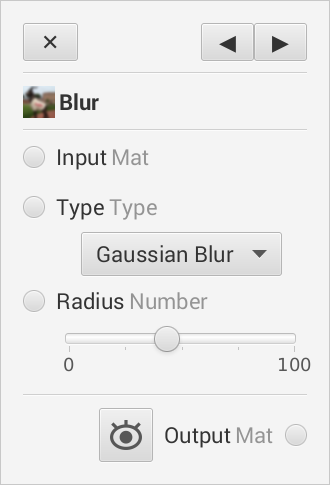
\includegraphics[scale = 0.5]{step.png}
}

The following actions can be performed on a step:
\begin{itemize}
    \item \textbf{Delete} a step by pressing the \textbf{x} button.
    \item \textbf{Move} a step left or right in the pipeline by pressing the \textbf{left} and \textbf{right} buttons.
\end{itemize}

\subsection{Connections}
In practice, a computer vision pipeline consists of many steps, where the outputs of earlier steps are uses as some of the inputs to later steps.  To represent this, we show "connections" between outputs and inputs of different steps, which are depicted as curved wires.\\

Connections can connect values such as images, which are not set with a user interface control, as well as primitive values such as numbers.  In the latter case, the UI control to set that value is disabled as long as the connection exists.  However, the most common case is the former, since computer vision algorithms typically involve performing many steps on an image.\\[0.5 cm]

\centerline{
    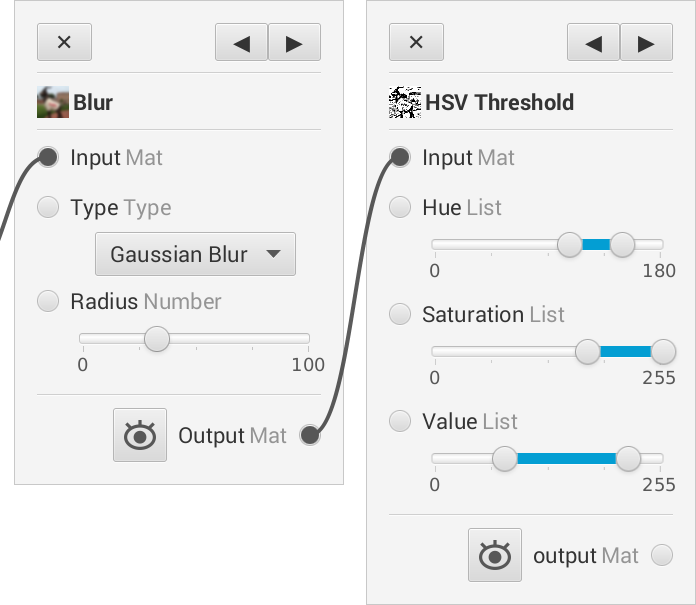
\includegraphics[scale = 0.5]{connection.png}
}

These actions can be preormed by the user to manipulate connections:
\begin{itemize}
    \item \textbf{Create} a connection by dragging and dropping an input to an output, or vice versa.
    \item \textbf{Delete} a connection by clicking one of the two handles.
\end{itemize}

\fxnote{We should explain how the UI works and show some screenshots}


%%%%%%%%%%%%%%%%%%%%%%%%%%%%%%%%%%%%%%%%%%%%%%%%%%%%%%%%%%%%%%%%%%%%%%%%%%%%%%%%%%%%%%%%%

\section{Schedule}
\fxnote{The timeline for stuff completed (or to be completed) for the project.  We should also talk about the FRC beta and how we put prioritized certain tasks in order to get feedback from FRC teams}

%%%%%%%%%%%%%%%%%%%%%%%%%%%%%%%%%%%%%%%%%%%%%%%%%%%%%%%%%%%%%%%%%%%%%%%%%%%%%%%%%%%%%%%%%

\section{Conclusion}

%%%%%%%%%%%%%%%%%%%%%%%%%%%%%%%%%%%%%%%%%%%%%%%%%%%%%%%%%%%%%%%%%%%%%%%%%%%%%%%%%%%%%%%%%

\newpage
\bibliographystyle{plain}
\bibliography{biblist}

\end{document}
